\documentclass[12pt]{article}
\usepackage{worksheet-common}

\begin{document}

\worksheettitle{Electric Field Superposition Practice}

%============================================================
\partsec{A}{Separation Vectors to a Field Point}

\prob A charge $q_1=+4.0\,\text{nC}$ sits at the origin. Find the vector $\vec{r}_1$ from $q_1$ to the point $P=(6.0\text{ cm},0)$, and its magnitude $|\vec{r}_1|$.

\begin{center}
\begin{tikzpicture}[x=0.32cm,y=0.32cm]
\draw[gray,->] (-1,0) -- (9,0) node[right] {$x$ (cm)};
\poscharge{0}{0}{1.3}
\node[below=5pt] at (0,-0.9) {$q_1=+4.0\,\text{nC}$};
\draw[dashed,brown] (0,0) -- (6,0);
\node[circle,draw,fill=white,inner sep=1.5pt] at (6,0) {};
\node[above=4pt] at (6,0) {$P$};
\end{tikzpicture}
\end{center}

\worksp{md}

\prob A charge $q_1=-2.0\,\text{nC}$ sits at $(2.0\text{ cm},3.0\text{ cm})$. Find $\vec{r}_1$ from $q_1$ to the point $P=(6.0\text{ cm},6.0\text{ cm})$, and $|\vec{r}_1|$.

\worksp{md}

\prob A charge $q_1=+250$ nC sits at the origin. Find $\vec{r}_1$ from $q_1$ to the point $P=(40\text{ mm},30\text{ mm})$, and $|\vec{r}_1|$, in meters.

\begin{center}
\begin{tikzpicture}[x=0.11cm,y=0.11cm]
\draw[gray,->] (0,0) -- (55,0) node[right] {$x$ (mm)};
\draw[gray,->] (0,0) -- (0,45) node[above] {$y$ (mm)};
\draw[dashed,brown] (0,0) -- (40,30);
\poscharge{0}{0}{3.2}
\node[below=2pt] at (0,-3.2) {$q_1=+250$ nC};
\node[circle,draw,fill=white,inner sep=1.5pt] at (40,30) {};
\node[above right=1pt] at (40,30) {$P=(40,30)$ mm};
\end{tikzpicture}
\end{center}

\worksp{md}

\prob A charge $q_1=-1.0\times10^{-6}$ C sits at $(5.0\times10^{-3}\text{ m},0)$. Find $\vec{r}_1$ from $q_1$ to the point $P=(0,1.2\times10^{-2}\text{ m})$, and $|\vec{r}_1|$.

\worksp{md}

\clearpage
%============================================================
\partsec{B}{Separation Vectors, Multiple Charges to One Point}

\prob Three charges: $q_1=+2.0\,\mu\text{C}$ at $(0,0)$, $q_2=-3.0\,\mu\text{C}$ at $(4.0\text{ cm},0)$, $q_3=+1.0\,\mu\text{C}$ at $(0,3.0\text{ cm})$. All three contribute to the field at $P=(4.0\text{ cm},3.0\text{ cm})$. Find $\vec{r}_1$, $\vec{r}_2$, and $\vec{r}_3$ (each charge to $P$), and their magnitudes.

\begin{center}
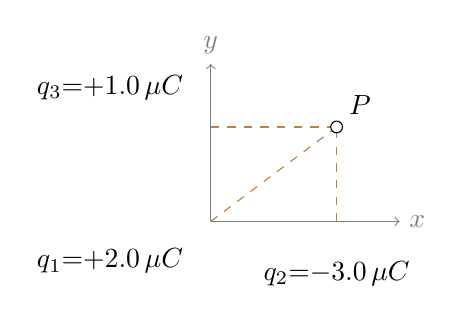
\begin{tikzpicture}[x=0.4cm,y=0.4cm]
\draw[gray,->] (0,0) -- (6,0) node[right] {$x$};
\draw[gray,->] (0,0) -- (0,5) node[above] {$y$};
\draw[dashed,brown] (0,0) -- (4,3);
\draw[dashed,brown] (4,0) -- (4,3);
\draw[dashed,brown] (0,3) -- (4,3);
\poscharge{0}{0}{1.0}
\node[below left=3pt] at (-0.3,-0.3) {$q_1{=}{+}2.0\,\mu\text{C}$};
\negcharge{4}{0}{1.0}
\node[below=4pt] at (4,-0.6) {$q_2{=}{-}3.0\,\mu\text{C}$};
\poscharge{0}{3}{1.0}
\node[above left=3pt] at (-0.3,3.3) {$q_3{=}{+}1.0\,\mu\text{C}$};
\node[circle,draw,fill=white,inner sep=1.5pt] at (4,3) {};
\node[above right=1pt] at (4,3) {$P$};
\end{tikzpicture}
\end{center}

\worksp{xl}

\prob Two charges: $q_1=+150$ nC at $(0,0)$, $q_2=-80$ nC at $(30\text{ mm},0)$. Both contribute to the field at $P=(30\text{ mm},40\text{ mm})$. Find $\vec{r}_1$ and $\vec{r}_2$, and their magnitudes.

\worksp{lg}

\prob \textbf{3D.} Two charges: $q_1=+5.0\,\text{nC}$ at the origin $(0,0,0)$, $q_2=-4.0\,\text{nC}$ at $(5.0\text{ cm},0,0)$. Both contribute to the field at $P=(0,4.0\text{ cm},3.0\text{ cm})$. Find $\vec{r}_1$ and $\vec{r}_2$ (each as an $(x,y,z)$ triple), and their magnitudes.

\worksp{lg}

\prob \textbf{3D.} Three charges: $q_1=+90$ nC at $(1.0\times10^{-2}\text{ m},0,0)$, $q_2=-60$ nC at $(0,2.0\times10^{-2}\text{ m},0)$, $q_3=+45$ nC at $(0,0,2.0\times10^{-2}\text{ m})$. All three contribute to the field at the origin $P=(0,0,0)$. Find $\vec{r}_1$, $\vec{r}_2$, and $\vec{r}_3$, and their magnitudes.

\worksp{lg}

\clearpage
%============================================================
\partsec{C}{Electric Field Magnitude \& Direction}

\textit{Same four single-charge setups as Part A. Use $E=k|q|/r^2$, along with $\vec{r}_1$ from Part A, to get the field at $P$ as a magnitude and a direction. (Careful with sign: the field of a negative charge points \emph{toward} it, not along $\vec{r}_1$.)}

\prob Same as \probref{1}: $q_1=+4.0$ nC, $P$ a distance $|\vec{r}_1|=6.0$ cm away along $+x$. Find the magnitude and direction of $\vec{E}_1$ at $P$.

\worksp{md}

\prob Same as \probref{2}: $q_1=-2.0$ nC, $\vec{r}_1=(4.0,3.0)$ cm. Find the magnitude and direction of $\vec{E}_1$ at $P$.

\worksp{md}

\prob Same as \probref{3}: $q_1=+250$ nC, $\vec{r}_1=(40,30)$ mm. Find the magnitude and direction of $\vec{E}_1$ at $P$.

\worksp{md}

\prob Same as \probref{4}: $q_1=-1.0\times10^{-6}$ C, $\vec{r}_1=(-5.0,12)\times10^{-3}$ m. Find the magnitude and direction of $\vec{E}_1$ at $P$.

\worksp{md}

\clearpage
%============================================================
\partsec{D}{Individual Field Vectors --- Components}

\textit{Same setups as Part B. Find the individual field $\vec{E}_i$ due to each charge alone at $P$, in component form. Don't add them together yet.}

\prob Same as \probref{5}: $q_1=+2.0\,\mu\text{C}$ at $(0,0)$, $q_2=-3.0\,\mu\text{C}$ at $(4.0,0)$ cm, $q_3=+1.0\,\mu\text{C}$ at $(0,3.0)$ cm; $P=(4.0,3.0)$ cm. Find $\vec{E}_1$, $\vec{E}_2$, and $\vec{E}_3$ at $P$, in component form.

\worksp{xl}

\prob Same as \probref{6}: $q_1=+150$ nC at $(0,0)$, $q_2=-80$ nC at $(30,0)$ mm; $P=(30,40)$ mm. Find $\vec{E}_1$ and $\vec{E}_2$ at $P$, in component form.

\worksp{xl}

\clearpage

\prob \textbf{3D.} Same as \probref{7}: $q_1=+5.0$ nC at $(0,0,0)$, $q_2=-4.0$ nC at $(5.0\text{ cm},0,0)$; $P=(0,4.0,3.0)$ cm. Find $\vec{E}_1$ and $\vec{E}_2$ at $P$, in component form.

\worksp{xl}

\prob \textbf{3D.} Same as \probref{8}: $q_1=+90$ nC at $(1.0,0,0)\times10^{-2}$ m, $q_2=-60$ nC at $(0,2.0,0)\times10^{-2}$ m, $q_3=+45$ nC at $(0,0,2.0)\times10^{-2}$ m; $P$ at the origin. Find $\vec{E}_1$, $\vec{E}_2$, and $\vec{E}_3$ at $P$, in component form.

\worksp{xl}

\clearpage
%============================================================
\partsec{E}{Net Field --- Superposition}

\textit{Add the individual fields from Part D as vectors to get the total field $\vec{E}_{\text{net}}$ at $P$. For the 2D setups, report components, magnitude, and direction. For the 3D setups, report components and magnitude only.}

\prob Using your answers from \probref{9}, find $\vec{E}_{\text{net}}$ at $P$ (components, magnitude, and direction).

\worksp{xl}

\prob Using your answers from \probref{10}, find $\vec{E}_{\text{net}}$ at $P$ (components, magnitude, and direction).

\worksp{lg}

\prob \textbf{3D.} Using your answers from \probref{11}, find $\vec{E}_{\text{net}}$ at $P$ (components and magnitude only).

\worksp{lg}

\prob \textbf{3D.} Using your answers from \probref{12}, find $\vec{E}_{\text{net}}$ at $P$ (components and magnitude only). This is the hardest one on the sheet --- nice work getting here.

\worksp{lg}

%============================================================
\begin{answerkey}
\begin{multicols}{2}

\akpart{Part A --- Separation Vectors to $P$}
\akitem{1}{$\vec{r}_1=(6.0,0)$ cm; $|\vec{r}_1|=6.0$ cm}
\akitem{2}{$\vec{r}_1=(4.0,3.0)$ cm; $|\vec{r}_1|=5.0$ cm}
\akitem{3}{$\vec{r}_1=(40,30)$ mm; $|\vec{r}_1|=50$ mm $=0.050$ m}
\akitem{4}{$\vec{r}_1=(-5.0,12)\times10^{-3}$ m; $|\vec{r}_1|=1.3\times10^{-2}$ m}

\vspace{2mm}
\akpart{Part B --- Separation Vectors, Multiple Charges}
\akitem{5}{$\vec{r}_1=(4.0,3.0)$cm, $|{\cdot}|=5.0$cm $\cdot$ $\vec{r}_2=(0,3.0)$cm, $|{\cdot}|=3.0$cm $\cdot$ $\vec{r}_3=(4.0,0)$cm, $|{\cdot}|=4.0$cm}
\akitem{6}{$\vec{r}_1=(30,40)$mm, $|{\cdot}|=50$mm $\cdot$ $\vec{r}_2=(0,40)$mm, $|{\cdot}|=40$mm}
\akitem{7}{(3D) $\vec{r}_1=(0,4.0,3.0)$cm, $|{\cdot}|=5.0$cm $\cdot$ $\vec{r}_2=(-5.0,4.0,3.0)$cm, $|{\cdot}|=7.07$cm}
\akitem{8}{(3D) $\vec{r}_1=(-1.0,0,0)$cm, $|{\cdot}|=1.0$cm $\cdot$ $\vec{r}_2=(0,-2.0,0)$cm, $|{\cdot}|=2.0$cm $\cdot$ $\vec{r}_3=(0,0,-2.0)$cm, $|{\cdot}|=2.0$cm}

\vspace{2mm}
\akpart{Part C --- Field Magnitude \& Direction}
\akitem{9}{$E_1=1.0\times10^4$ N/C, along $+x$}
\akitem{10}{$E_1=7.19\times10^3$ N/C, $36.9^\circ$ below $-x$ (toward $q_1$)}
\akitem{11}{$E_1=8.99\times10^5$ N/C, $36.9^\circ$ above $+x$}
\akitem{12}{$E_1=5.32\times10^7$ N/C, $67.4^\circ$ below $+x$ (toward $q_1$)}

\vspace{2mm}
\akpart{Part D --- Individual Fields at $P$}
\akitem{13}{$\vec{E}_1=(5.75,4.32)\times10^6$ N/C $\cdot$ $\vec{E}_2=(0,-3.00\times10^7)$ N/C $\cdot$ $\vec{E}_3=(5.62\times10^6,0)$ N/C}
\akitem{14}{$\vec{E}_1=(3.24,4.32)\times10^5$ N/C $\cdot$ $\vec{E}_2=(0,-4.50\times10^5)$ N/C}
\akitem{15}{(3D) $\vec{E}_1=(0,1.44,1.08)\times10^4$ N/C $\cdot$ $\vec{E}_2=(5.09,-4.07,-3.05)\times10^3$ N/C}
\akitem{16}{(3D) $\vec{E}_1=(-8.09,0,0)\times10^6$ N/C $\cdot$ $\vec{E}_2=(0,1.35,0)\times10^6$ N/C $\cdot$ $\vec{E}_3=(0,0,-1.01)\times10^6$ N/C}

\vspace{2mm}
\akpart{Part E --- Net Field at $P$}
\akitem{17}{$\vec{E}_{\text{net}}=(1.14,-2.57)\times10^7$ N/C; $|\vec{E}_{\text{net}}|=2.81\times10^7$ N/C, $66.1^\circ$ below $+x$}
\akitem{18}{$\vec{E}_{\text{net}}=(3.24\times10^5,-1.80\times10^4)$ N/C; $|\vec{E}_{\text{net}}|=3.24\times10^5$ N/C, $3.2^\circ$ below $+x$}
\akitem{19}{(3D) $\vec{E}_{\text{net}}=(5.09,10.3,7.74)\times10^3$ N/C; $|\vec{E}_{\text{net}}|=1.39\times10^4$ N/C}
\akitem{20}{(3D) $\vec{E}_{\text{net}}=(-8.09,1.35,-1.01)\times10^6$ N/C; $|\vec{E}_{\text{net}}|=8.26\times10^6$ N/C}

\end{multicols}
\end{answerkey}

\end{document}
